\chapter{Modelo de Dados}

O modelo de dados foi feito para ser o mais simples possível para que futuras alterações
possam ser feitas facilmente. Abaixo está o diagrama entidade-relacionamento no qual
o nome no topo do retângulo identifica o nome da tabela. A lista abaixo mostra
as colunas dessas tabelas, com um ícone de uma chave preta para a \textit{chave primária} e 
uma chave verde para a \textit{chave estrangeira}.

Uma relação é denotada pelas setas ligando duas tabelas. A cardinalidade da relação é indicada
pelos números entre parênteses. 

Para a relação \texttt{Aerodrome-ILS}, temos (1, 1) para (0, n), significando que um aeródromo pode
ter zero ou mais frequências de ILS e esta só pode ser de um único aeródromo.

Já na relação \texttt{Aerodrome} com \texttt{Runway}, um aeródromo deve ter \texttt{uma ou mais} pistas.


\begin{figure}[ht]
    \begin{center}
    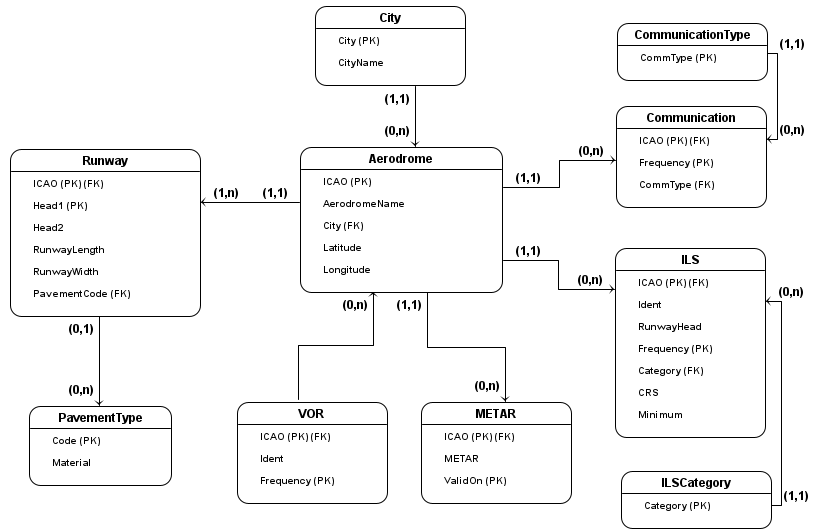
\includegraphics[width=400pt]{img/ERAero.png}
    \caption{Diagrama E/R}
    \label{fig:diagrama-er}
    \end{center}
\end{figure}

Note que as tabelas "CommunicationType", "ILSCategory" e "PavementType" poderiam ser substituídas
por colunas enum nas tabelas "Communication", "ILS" e "Runway", porém a manutenção seria difícil
\cite{table-enum},
pois teríamos que alterar a estrutura das tabelas (possívelmente tirando o sistema do ar) caso 
fosse necessário adicionar um tipo novo
de comunicação, por exemplo. Fazendo com uma tabela externa é necessário apenas adicionar uma nova
linha.

\section{TABELA: City}
\subsection{CityName (PK)}

Nome da cidade escrito em Português com a primeira letra maiúscula.


\section{TABELA: Aerodrome}

A tabela central para todas as outras, contém informações sobre o aeroporto ou aeródromo. 
Já que o segundo termo é mais geral que o primeiro, preferi usar este.

\subsection{ICAO (PK)}
O código ICAO do aeródromo emitido pela Organização Internacional de Aviação Civil 
(International Civil Aviation Organization). Por ser único, pode ser usado como chave primária.

\subsection{AerodromeName}
O nome do aeródromo conforme definido pelo AISWEB, sistema nacional de informações aeronáuticas.

\subsection{City}
Nome da cidade escrito em Português. A primeira letra é maiúscula.
Chave estrangeira para a tabela \texttt{City}.

\subsection{Latitude}
A latitude do aeroporto em graus no formato de graus decimais (DD, Decimal Degrees). Três dígitos 
para representar a parte inteira e seis dígitos para a fracionária.

\subsection{Longitude}
A longitude do aeroporto, seguindo o mesmo formato da latitude.

\subsection{METAR}
O METAR válido atualmente para este aeródromo. Considerei colocar o METAR como tabela separada
com chave estrangeira para o aerodrómo para, deste modo, ter o METAR histórico. Mas, no 
contexto de planejamento de voo, os METARs anteriores não possuem muita serventia.

\section{TABELA: PavementType}

Material da superfície da pista, como asfalto, concreto, brita e outros.

\subsection{Code}
O código (em Inglês) do tipo de pavimento usado. É formado por três letras maiúsculas.

\subsection{Material}
O nome do pavimento em Português, com a primeira letra maiúscula.

\begin{verbatim}
Exemplo de tabela:

Code    Material
ASP     Asfalto
CON     Concreto
GVL     Brita
\end{verbatim}


\section{TABELA: Runway}

É importante conhecer as características dos tipos de pistas de 
pouso e decolagem, pois seu comprimento determinará a quantidade de freio 
necessária para parar uma determinada aeronave.

Se a pista for muito curta, determinados modelos de avião não poderão pousar. 
A largura da pista determina a envergadura máxima que uma aeronave pode ter 
para operar nessa pista. Se uma pista for muito estreita, uma aeronave quadrimotora 
como o Boeing 747 pode sofrer ingestão de materiais, já que os dois motores mais 
externos ficarão para fora da área da pista, sobre o gramado.

\subsection{ICAO (FK e PK)}

O código ICAO do aeródromo ao qual a pista está associada, utilizado como chave estrangeira 
fazendo a ligação com a tabela 'Aerodrome'.

\subsection{Head1 (PK)}

Número e possível letra que identifica uma das cabeceiras da pista. Um aeroporto nunca terá
cabeceiras repetidas, então ICAO e Head1 formam uma chave primária mínima.

Para cabeceiras paralelas, ou seja, que apontam para a mesma direção, temos:

\subsubsection{Pista única}

A proa em que a pista aponta, com divisão por 10 arredondada. Por exemplo, em Fortaleza,
temos uma cabeceira com curso de 126 graus, dividindo por 10 temos 12,6, arredondando
temos o número 13 da cabeceira.

\subsubsection{Pista dupla}

Para duas pistas paralelas, usamos L para a cabeceira da esquerda e R para a da direita.
Por exemplo, no Santos Dumont, de costas para o Pão de Açúcar, temos as cabeceiras 02L 
(na esquerda) e 02R (na direita).

\subsubsection{Pista tripla}

Não temos aeroportos com três pistas paralelas no Brasil, mas são usadas as letras
L, C e R. C para a pista central.

\subsection{Head2}

Número e possível letra que identifica a outra cabeceira da mesma pista.

\subsection{RunwayLength}

Comprimento da pista em metros.

\subsection{RunwayWidth}

Largura da pista em metros.

\subsection{PavementCode (FK)}

O tipo de pavimento da pista, referenciando a tabela 'PavementType'.


\section{TABELA: CommunicationType}

Esta tabela define os diferentes tipos de comunicação disponíveis em um aeródromo.

\subsection{CommType}
O tipo de comunicação, podendo ser "Torre", "Solo", "ATIS", "Tráfego" ou "Operação".


\section{TABELA: Communication}

Esta tabela guarda as frequências de comunicação utilizadas em um aeródromo. As 
freqências de radionavegação são colocadas nas tabelas "ILS" e "VOR".

\subsection{ICAO (FK e PK)}
O código ICAO do aeródromo ao qual a frequência de comunicação está associada, utilizado 
como chave estrangeira referenciando a tabela 'Aerodrome'.

\subsection{Frequency (PK)}
A frequência em MHz. ICAO e frequency formam chave primária. Note que uma frequência,
não é única em todo o país, para distâncias longas, onde não há risco de interferência,
é possível haverem frequências repetidas.

\subsection{CommType (FK)}
O tipo de comunicação, chave estrangeira para 'CommunicationType'.


\section{TABELA: ILSCategory}

Esta tabela lista as diferentes categorias de Sistema de Pouso por Instrumentos
 (Instrument Landing System).

\subsection{Category}

A categoria de ILS, sendo "CAT I", "CAT II", "CATIIIA", "CATIIIB" ou
 "CAT IIIC". Será explicado melhor em "Minimus" na tabela "ILS".

\section{TABELA: ILS}

Esta tabela descreve os Sistemas de Pouso por Instrumentos (Instrument
Landing System) disponíveis no aeródromo.

\subsection{ICAO (FK e PK)}

O código ICAO do aeródromo ao qual o sistema de pouso está associado, utilizado 
como chave estrangeira referenciando a tabela 'Aerodrome'.

\subsection{Ident (PK)}

Identificação de três letras maisculas única do ILS para aquele aeródromo.
Junto com ICAO formam a chave primária. Como no caso da comunicação, é
possível haverem duas Ident iguas desde que não estejam próximas.

\subsection{Frequency}

A frequência de operação do ILS em MHz.

\subsection{Category (FK)}

A categoria do ILS, referenciando a tabela 'ILSCategory'.

\subsection{CRS}

A referência do curso de aproximação do ILS. É a proa final que a aeronave deve 
manter para o correto alinhamento nesta cabeceira.

\subsection{Minimum}

A altura mínima de decisão em pés para operação do ILS. A partir desta altura, é
desligado o piloto automático e o resto da aproximação é feita manualmente.
Se a altitude da aeronave ficar abaixo deste valor e ainda não for possível 
ter visual da pista é obrigatória a arremetida.

Quando maior a categoria do ILS, maior a precisão do sistema, portanto a Minimus 
será mais baixa. Uma "CAT IIIC" (pronuncia-se cat três charlie), possui Minimus zero, 
portanto a aeronave pode pousar de forma totalmente automática.

\section{TABELA: VOR}

Esta tabela registra os sistemas de navegação VOR/DME disponíveis em um aeródromo.
Não foi incluída uma tabela para as frequências de NDB porque este sistema
está caíndo em desuso.

\subsection{Ident}
Identificação única do VOR/DME para aquele aeródromo.

\subsection{ICAO}
O código ICAO do aeródromo ao qual o VOR/DME está associado, utilizado como 
chave estrangeira referenciando a tabela 'Aerodrome'.

\subsection{Frequency}
A frequência de operação do VOR/DME em MHz.